\subsection{The geometric significance of the dot product}

The \textbf{included angle}\index{included angle} of two vectors
$\vect{u}$ and $\vect{v}$ is the angle $\theta$ between the vectors
such that $0 \leq \theta \leq \pi$.
\begin{center}
  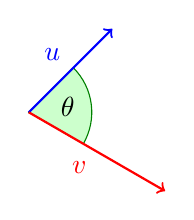
\begin{tikzpicture}
    \filldraw[fill=green!20,draw=green!50!black] (0,0) -- (-30:8mm) arc (-30:45:8mm) -- cycle;
    \draw[->, thick, blue](0,0) -- node[above left] {$\vect{u}$} (45:1.5);
    \draw[->, thick, red](0,0) -- node[below left] {$\vect{v}$} (-30:2);
    \node at (7.5:5mm){$\theta$};
  \end{tikzpicture}
\end{center}
The dot product can be used to determine the included angle between
two vectors.

\begin{proposition}{The dot product and the included angle}{dot-product-angle}
  Let $\vect{u}$ and $\vect{v}$ be two vectors in $\R^n$, and let
  $\theta$ be the included angle. Then the following equation holds.
  \begin{equation*}
    \vect{u}\dotprod \vect{v}=\norm{\vect{u}} \norm{\vect{v}} \cos \theta.
  \end{equation*}
\end{proposition}

In words, the dot product of two vectors equals the product of the
magnitude (or length) of the two vectors multiplied by the cosine of
the included angle. Note that this gives a geometric description of
the dot product that does not depend explicitly on the coordinates of
the vectors.

\begin{example}{Find the angle between two vectors}{angle-two-vectors}
  Find the angle%
  \index{angle!between vectors} between the vectors
\begin{equation*}
  \vect{u}
  =
  \begin{mymatrix}{r}
    2 \\
    2
  \end{mymatrix}
  \quad\mbox{and}\quad
  \vect{v}
  =
  \begin{mymatrix}{r}
    0 \\
    3
  \end{mymatrix}.
\end{equation*}
\end{example}

\begin{solution}
  By Proposition~\ref{prop:dot-product-angle},
  \begin{equation*}
    \vect{u}\dotprod \vect{v}=\norm{\vect{u}} \norm{\vect{v}} \cos \theta.
  \end{equation*}
  Hence,
  \begin{equation*}
    \cos \theta =\frac{\vect{u}\dotprod \vect{v}}{\norm{\vect{u}}\norm{\vect{v}}}.
  \end{equation*}
  First, we compute $\vect{u}\dotprod \vect{v} = (2)(0) + (2)(3) = 6$.
  Then,
  \begin{equation*}
    \begin{array}{l}
      \norm{\vect{u}} = \sqrt{2^2+2^2}=\sqrt{8},\\
      \norm{\vect{v}} = \sqrt{0^2+3^2}=3.
    \end{array}
  \end{equation*}
  Therefore, we have
  \begin{equation*}
    \cos \theta =\frac{6}{3\sqrt{8}} = \frac{1}{\sqrt{2}}.
  \end{equation*}
  Taking the inverse cosine of both sides of the equation, we find
  that $\theta =\frac{\pi}{4}$ radians, or 45 degrees.
\end{solution}

\begin{example}{Computing a dot product from an angle}{geometric-dot-product}
  Let $\vect{u},\vect{v}$ be vectors with $ \norm{\vect{u}} = 3$ and $\norm{\vect{v}} = 4$.
  Suppose the angle between $\vect{u}$ and $\vect{v}$ is $\pi / 3$. Find $\vect{u}\dotprod \vect{v}$.
\end{example}

\begin{solution}
  From Proposition~\ref{prop:dot-product-angle}, we have
  \begin{equation*}
    \vect{u}\dotprod \vect{v}
    =\norm{\vect{u}} \norm{\vect{v}} \cos \theta
    =3\cdot 4\cdot \cos\paren{\frac{\pi}{3}}
    =3\cdot 4\cdot \frac{1}{2}=6.
\end{equation*}
\end{solution}

